From the above section, it is easy to see that, with different CPU frequency, both stretched replication and shadow replication can have different response time, task reliability, and energy consumption. In order to derive the frequency for stretched replication and shadow replication respectively, we come up with the following problem: Given a task and its task reliability target, determine the frequency assignment such that the energy consumption is minimized while guarantee that the task can be completed before its deadline with required reliability. 

\subsection{Problem formulation}
Assuming CPU frequency is continuous, the problem can be mathematically formulated as:

\begin{align}
\min_{\sigma}\quad\quad    & E \\
s.t.              \quad\quad                   & \sigma_{min} \leq \sigma \leq \sigma_{max} \\
                                     & T \leq P \\
                                     & R \leq R_{target} 
\end{align} 

%\begin{equation}
%\label{optimization_problem}
%%\setlength{\abovedisplayskip}{14pt}
%\begin{alignedat}{2}
%\min_{\sigma}    & E \\
%s.t.                                 & \sigma_{min} \leq \sigma \leq \sigma_{max} \\
%                                     & T \leq P \\
%                                     & R_{target} \leq R 
%\end{alignedat}
%\end{equation}

Above, Equation (1) says the objective is to minimize energy consumption. Constraint (2) ensures a valid frequency is used for each task instance. For stretched replication, $\sigma_r$ need to satisfy this requirement, and for shadow replication, $\sigma_m$, $\sigma_b$, and $\sigma_a$ all need to satisfy this condition. Constraint (3) says the task's completion time should be earlier than the deadline. For shadow replication, this is equivalent to that the shadow can complete before deadline. The last constraint specifies that the task failure probability should be low enough to satisfy the reliability requirement. 

\subsection{Analysis}
We programmed the energy-optimal replication problem with MatLab and used the nonlinear optimization algorithms implemented in MatLab to solve the problem. However, this approach is quite time-consuming. It takes more than half an hour to solve one instance of the problem. Therefore, we decide to take another path that uses brute force search to find out the optimal frequency assignment. This approach ended up to be much faster than the first approach, as a processor should only have a few valid frequency choices. 

Below we show some results in Fig.~\ref{fig:failure_impact} and Fig.~\ref{fig:utilization_impact}. Fig.~\ref{fig:en_failure_10_100} shows the energy consumption comparison among the three replication techniques for different reliability requirement in terms of task failure probability.The parameters are adopted from~\cite{6604518} and shown in the figure title. With two replicas under the specified parameters, the lowest task failure probability that can be achieved is $10^{-10}$, which is the rightmost point in the figure.  
All the results are normalized to the energy consumption of naive replication. It is clear that both stretched replication and shadow replication consume less energy than naive replication. When target task failure probability is high (left side of the figure), both stretched replication and shadow replication are able to slow down to a large extent and achieve the most energy saving compared to naive replication. As target task failure probability increases, the space for slowing down decreases. As a result, the energy saving decreases as well. At the highest reliability requirement, both stretched replication and shadow replication are forced to use the maximum frequency, i.e., they converge to naive replication. Compared to stretched replication, shadow replication is able to save 4\% to 10\% of energy. The frequency assignment to achieve the optimal energy for stretched replication and shadow replication are shown in Fig.~\ref{fig:speed_failure_10_100}. As we described above, the assigned frequency increases as the reliability requirement increases, except for $\sigma_a$ that always uses the maximum frequency.

\begin{figure}[!t]
	\begin{center}
		\subfigure[Energy consumption]
		{
			\label{fig:en_failure_10_100}
			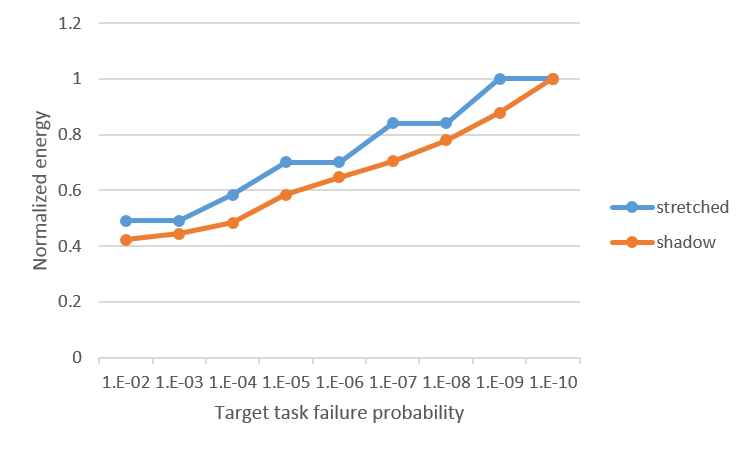
\includegraphics[width=0.45\columnwidth]{Figures/energy_vs_failure_10_100}
		} 
		\subfigure[CPU frequency]
		{
			\label{fig:speed_failure_10_100}
			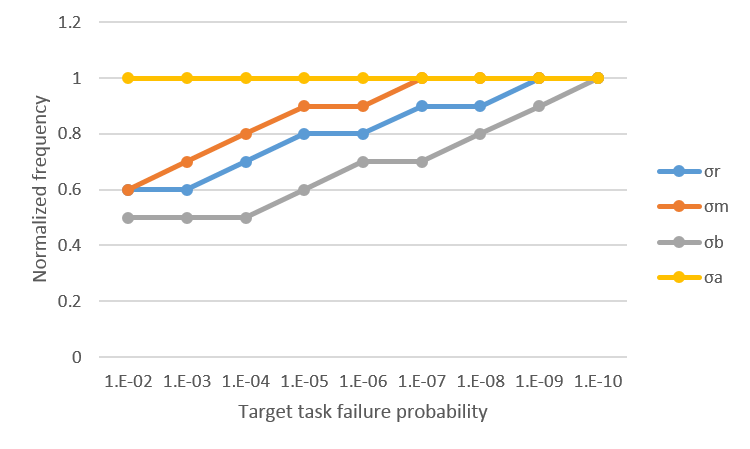
\includegraphics[width=0.45\columnwidth]{Figures/speed_vs_failure_10_100}
		} 
	\end{center}
	%\vskip -0.22in 
	\caption{Impact of target task failure probability on frequency assignment and energy consumption. $c=10ms$, $P=100ms$, $f_{min}=0.5$, $\alpha=0.1$, $d=4$, $\lambda_0=10^{-6}$.}
	\label{fig:failure_impact}
\end{figure}

\begin{figure}[!t]
	\begin{center}
		\subfigure[Energy consumption]
		{
			\label{fig:en_util_10}
			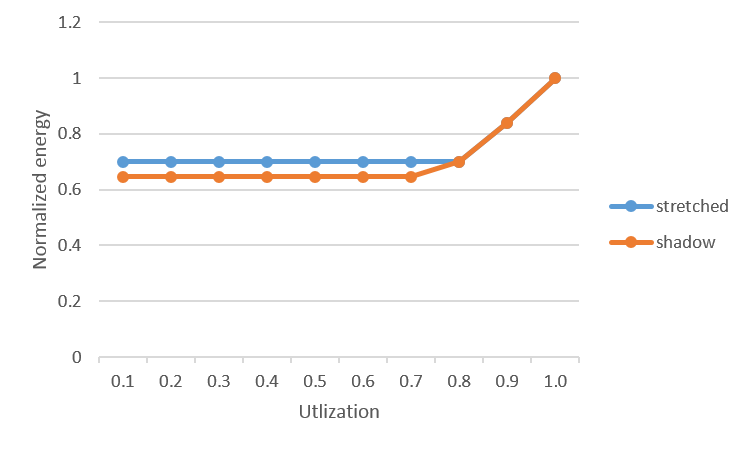
\includegraphics[width=0.45\columnwidth]{Figures/energy_vs_uti_10}
		} 
		\subfigure[CPU frequency]
		{
			\label{fig:speed_util_10}
			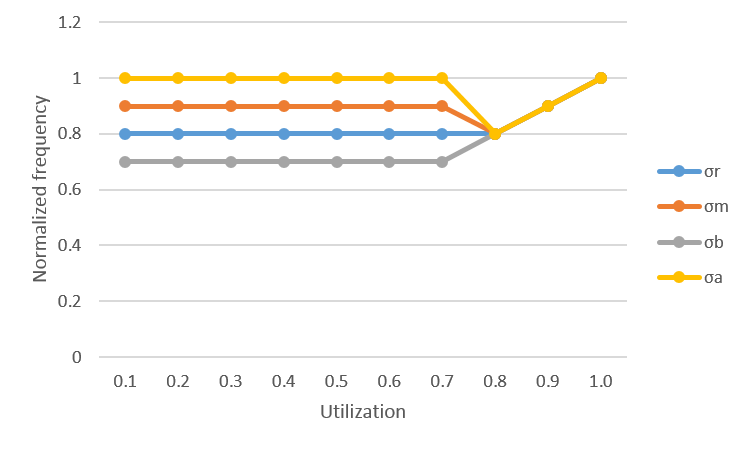
\includegraphics[width=0.45\columnwidth]{Figures/speed_vs_uti_10}
		} 
	\end{center}
	%\vskip -0.22in 
	\caption{Impact of utilization on frequency assignment and energy consumption. $c=10ms$, $R_{target}=10^{-6}$, $f_{min}=0.5$, $\alpha=0.1$, $d=4$, $\lambda_0=10^{-6}$.}
	\label{fig:utilization_impact}
\end{figure}

Fig.~\ref{fig:utilization_impact} shows the energy consumption and frequency assignment for different task utilizations. As expected, the right side of the figures show that the lower the utilization is, the larger space there is for slowing down, and the more energy saving there is for stretched replication and shadow replication. When utilization reaches 0.8, shadow replication converges to stretched replication. The energy and frequency are flat at the left side because the target task failure probability also restricts how much the tasks can slow down, as shown in Fig.~\ref{fig:failure_impact}. 
